\documentclass[crop,tikz]{standalone}

\tikzset{>=latex}
\newcommand{\place}{\vec{r}}
\newcommand{\F}{\vec{F}}
\colorlet{green}{black!40!green}

\begin{document}
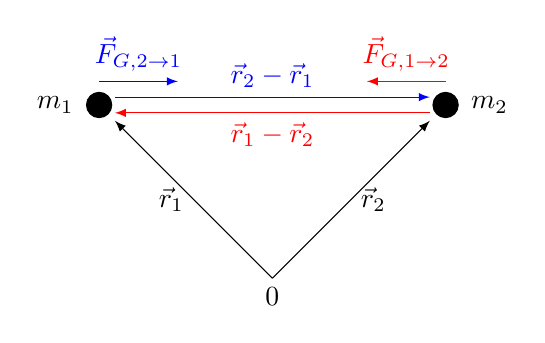
\begin{tikzpicture}[scale=2]
  \draw[->] (0,0) node[below] {$0$} -- node[left] {$\place_1$} (-1,1);
  \draw[->] (0,0) -- node[right] {$\place_2$} (1,1);
  \draw[fill,black] (-1,1)+(-0.1,0.1) circle (0.08);
  \draw[fill,black] (1,1)+(0.1,0.1) circle (0.08);
  \draw[->,blue] (-1,1.15) -- node[above] {$\place_2-\place_1$} (+1,1.15);
  \draw[->,red]  (+1,1.05) -- node[below] {$\place_1-\place_2$} (-1,1.05);
  \draw (-1.2,1.1) node[left] {$m_1$};
  \draw (1.2,1.1) node[right] {$m_2$};
  \draw[->,blue] (-1.1,1.25) -- node[above] {$\F_{G,2\to 1}$} +(+0.5,0);
  \draw[->,red]  (+1.1,1.25) -- node[above] {$\F_{G,1\to 2}$} +(-0.5,0);
\end{tikzpicture}
\end{document}
